\documentclass{article}
\usepackage{fancyhdr}
\usepackage[margin=1in]{geometry}
\usepackage{amsmath}
\usepackage{siunitx}
\usepackage{array}
\usepackage{pgfplots}
\usepackage{graphicx}


\pagestyle{fancy}
\fancyhf{}
\chead{Física Experimental III • Experimento realizado em 20/10/2023}
\rfoot{\thepage}
\renewcommand{\headrulewidth}{0.4pt}

\begin{document}

\begin{center}
    \huge
    \textbf{Tensões e Correntes Elétricas}
    \normalsize
    \vspace{10pt}

    Matheus Aparecido Souza Silva, Isabela Sant'Ana, Gustavo Peres, João Vitor Costa
    \vspace{5pt}

    \textbf{Turma}: TA \quad \textbf{Horário}: 6M45 \quad \textbf{Curso}: Engenharia Elétrica

\section{Coleta de dados:}
\subsection{Tabela de dados das medições de resistências}

\begin{tabular}{|c|c|c|c|}
    \hline
    Associação & Valor Nominal (\(\Omega\)) $\pm$ Tolerância & Valor Experimental (\(\Omega\)) $\pm$ Incerteza \\
    \hline
    R\textsubscript{1} & 47 $\pm$ 5\% & 46.70 $\pm$ 0.62 \\
    \hline
    R\textsubscript{2} & 220 $\pm$ 5\% & 218.8 $\pm$ 2.2 \\
    \hline
    R\textsubscript{3} & 120 $\pm$ 5\% & 120.9 $\pm$ 1.3 \\
    \hline
    R\textsubscript{e} (Série) & 387 $\pm$ 5\% & 386.4 $\pm$ 3.7 \\
    \hline
    R\textsubscript{e} (Paralelo) & 29.277 $\pm$ 5\% & 29.20 $\pm$ 0.46 \\
    \hline
    R\textsubscript{e} (Misto) & 94.935 $\pm$ 5\% & 94.9 $\pm$ 1.0 \\
    \hline 
\end{tabular}

\subsection{Tabela de dados experimentais}

\begin{tabular}{|c|c|c|c|c|}
    \hline
     & Resistores Individuais & Resistores em Série & Resistores em Paralelo & Associação Mista \\
    \hline
    $V_1 \pm \Delta V_1$ & $4.024 \pm 0.022$ & $0.491 \pm 0.004$ & $4.025 \pm 0.022 $ & $0.491 \pm 0.004 $\\
    \hline
    $V_2 \pm \Delta V_2$ & $4.028 \pm 0.022$ & $2.321 \pm 0.013$ & $4.029 \pm 0.022 $ & $3.544 \pm 0.019 $\\
    \hline
    $V_3 \pm \Delta V_3$ & $4.029 \pm 0.022$ & $1.223 \pm 0.008$ & $4.026 \pm 0.022 $ & $3.544 \pm 0.019 $\\
    \hline
    $V \pm \Delta V$ & $---$ & $4.035 \pm 0.022$ & $4.026 \pm 0.022 $ & $4.035 \pm 0.022 $\\
    \hline
    $i_1 \pm \Delta i_1$ & $0.087 \pm 0.004$ & $0.011 \pm 0.003$ & $0.086 \pm 0.004$ & \\
    \hline
    $i_2 \pm \Delta i_2$ & $0.018 \pm 0.003$ & $0.011 \pm 0.003$ & $0.019 \pm 0.003$ & \\
    \hline
    $i_3 \pm \Delta i_3$ & $0.035 \pm 0.003$ & $0.011 \pm 0.003$ & $0.036 \pm 0.003$ & \\
    \hline
    $i \pm \Delta i$ & $---$ & $0.011 \pm 0.003$ &$0.141 \pm 0.005$ & \\
    \hline
    $R_1 \pm \Delta R_1$ & $46.242 \pm 2.141$ & $44.63 \pm 12,178$ &$46.802 \pm 2.191$ & \\
    \hline
    $R_2 \pm \Delta R_2$ & $223.5 \pm 37.270$ & $211 \pm 57,546$ &$212.052 \pm 33,502$ & \\
    \hline
    $R_3 \pm \Delta R_3$ & $114.971 \pm 9.874$ & $118.18 \pm 32.240$ & $111.916 \pm 9.346$ & \\
    \hline
    $R_e \pm \Delta R_e$ & $---$ & $366,818 \pm 100.061$ & $28,553 \pm 1.069$ & \\
    \hline
\end{tabular}

\section{Atividades} 
    \subsection{Associação de resistores em série:}

    \begin{figure}[h]
        \centering
        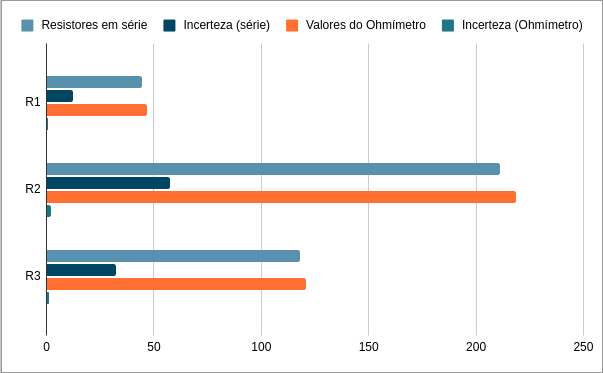
\includegraphics[width=0.5\textwidth]{Associação dos resistores em série.png}
      \end{figure}
    
      \subsection{Associação de resistores em paralelo:}

      \begin{figure}[h]
        \centering
        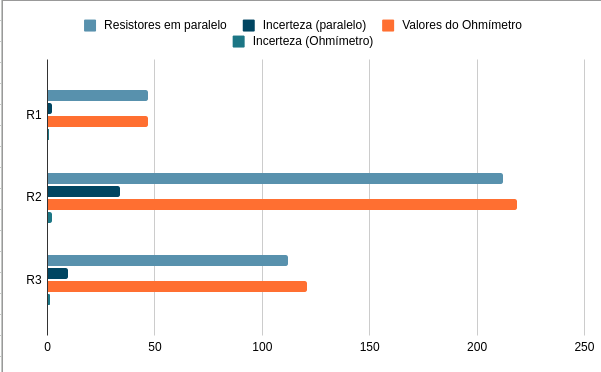
\includegraphics[width=0.5\textwidth]{Associação de resistores em paralelo.png}
      \end{figure}

\end{center}
\end{document}
